\chapter{Security Fundamentals}\label{security-fundamentals}

\section{Key Security Concepts}\label{key-security-concepts}

WHY SECURITY?

What is the purpose / goal of SECURITY in an ENTERPRISE ?

\begin{itemize}
\tightlist
\item
  The principles of the CIA TRIAD form the FOUNDATION of SECURITY:

  \begin{itemize}
  \tightlist
  \item
    CONFIDENTIALITY

    \begin{itemize}
    \tightlist
    \item
      Only AUTHORIZED USERS should be able to ACCESS DATA
    \item
      Some INFORMATION / DATA is PUBLIC and can be accessed by ANYONE
    \item
      Some INFORMATION / DATA is SECRET and should be only be accessed
      by SPECIFIC people
    \end{itemize}
  \item
    INTEGRITY

    \begin{itemize}
    \tightlist
    \item
      DATA should not be tampered with (modified) by unauthorized USERS
    \item
      DATA should be CORRECT and AUTHENTIC
    \end{itemize}
  \item
    AVAILABILITY

    \begin{itemize}
    \tightlist
    \item
      The NETWORK / SECURITY should be OPERATIONAL and ACCESSIBLE to
      AUTHORIZED USERS
    \end{itemize}
  \end{itemize}
\end{itemize}

ATTACKERS can threaten the CONFIDENTIALITY, INTEGRITY, and AVAILBILITY
of an enterprise's SYSTEMS and INFORMATION

\section{Vulnerability, Exploit, Threat,
Mitigation}\label{vulnerability-exploit-threat-mitigation}

\begin{itemize}
\tightlist
\item
  A VULNERABILITY is any potential weakness that can compromise the CIA
  of a SYSTEM / INFO

  \begin{itemize}
  \tightlist
  \item
    A potential weakness isn't a problem in its own
  \end{itemize}
\item
  AN EXPLOIT is something that can potentially be used to exploit the
  vulnerability

  \begin{itemize}
  \tightlist
  \item
    Something than can \emph{potentially} be used as an exploit isn't a
    problem on it's own.
  \end{itemize}
\item
  A THREAT is the potential of a VULNERABILITY to be EXPLOITED

  \begin{itemize}
  \tightlist
  \item
    A hacker EXPLOITING a VULNERABILITY in your system is a THREAT
  \end{itemize}
\item
  A MITIGATION TECHNIQUE is something that can protect against threats

  \begin{itemize}
  \tightlist
  \item
    Should be implemented everywhere a VULNERABILITY can be EXPLOITED:

    \begin{itemize}
    \tightlist
    \item
      Client Devices
    \item
      Servers, Switches, Routers, Firewalls
    \item
      etc.
    \end{itemize}
  \end{itemize}
\end{itemize}

\begin{tipbox}

NO SYSTEM IS PERFECTLY SECURE!

\end{tipbox}

\section{Common Attacks}\label{common-attacks}

\begin{itemize}
\tightlist
\item
  DoS (Denial of Service) Attacks
\item
  Spoofing Attacks
\item
  Reflection / Amplification Attacks
\item
  Man-in-the-Middle Attacks
\item
  Reconnaissance Attacks
\item
  Malware
\item
  Social Engineering Attacks
\item
  Password-Related Attacks
\end{itemize}

DoS (Denial of Service) Attacks

\begin{itemize}
\tightlist
\item
  DoS attacks threaten the AVAILABILITY of the SYSTEM
\item
  One common DoS attack is the TCP SYN Flood

  \begin{itemize}
  \tightlist
  \item
    TCP Three-Way Handshake : SYN \textbar{} SYN-ACK \textbar{} ACK
  \item
    The ATTACKER sends countless TCP SYN messages to the TARGET
  \item
    The TARGET sends a SYN-ACK message in response to each SYN it
    receives
  \item
    The ATTACKER never replies with the final ACK of the TCP Three-Way
    Handshake
  \item
    The incomplete connections fill up the TARGET'S TCP connection table
  \item
    The ATTACKER continues sending SYN messages
  \item
    The TARGET is no longer able to make legitimate TCP connections
  \end{itemize}
\end{itemize}

\begin{figure}
\centering
\pandocbounded{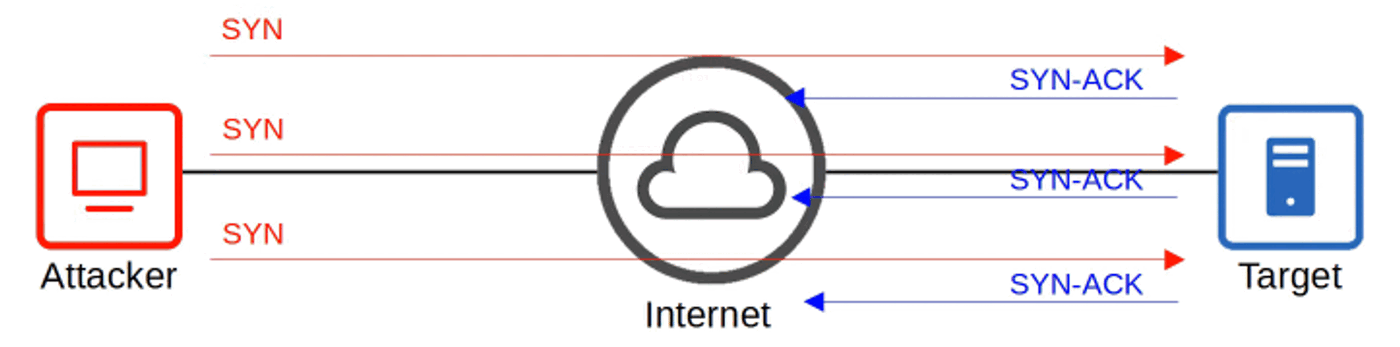
\includegraphics[keepaspectratio,alt={image}]{images/49-security-fundamentals/img-001.png}}
\end{figure}

\begin{itemize}
\tightlist
\item
  In a DDoS (Distributed Denial of Service) Attack, the ATTACKER infects
  many computers with MALWARE and uses them to initiate a
  Denial-of-Service Attack.
\item
  This group of infected computers is called a BOTNET
\end{itemize}

Example : A TCP SYN Flood Attack

\begin{figure}
\centering
\pandocbounded{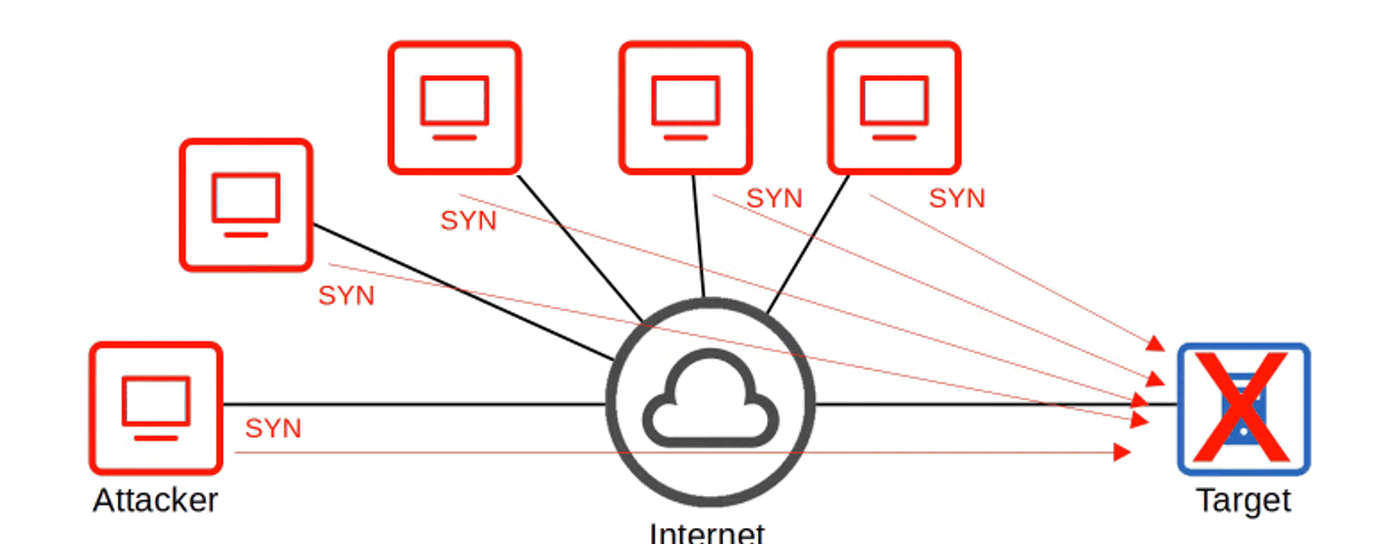
\includegraphics[keepaspectratio,alt={image}]{images/49-security-fundamentals/img-002.png}}
\end{figure}

\section{Spoofing Attacks}\label{spoofing-attacks}

\begin{itemize}
\tightlist
\item
  To SPOOF an ADDRESS is to use a FAKE SOURCE ADDRESS (IP or MAC)
\item
  Numerous attacks involve spoofing; it's not a SINGLE kind of attack
\item
  An example is a DHCP EXHAUSTION attack
\item
  An ATTACKER uses spoofed MAC ADDRESSES to flood DHCP Discover messages
\item
  The TARGET server's DHCP POOL becomes full, resulting in a
  Denial-of-Service to other DEVICES
\end{itemize}

\begin{figure}
\centering
\pandocbounded{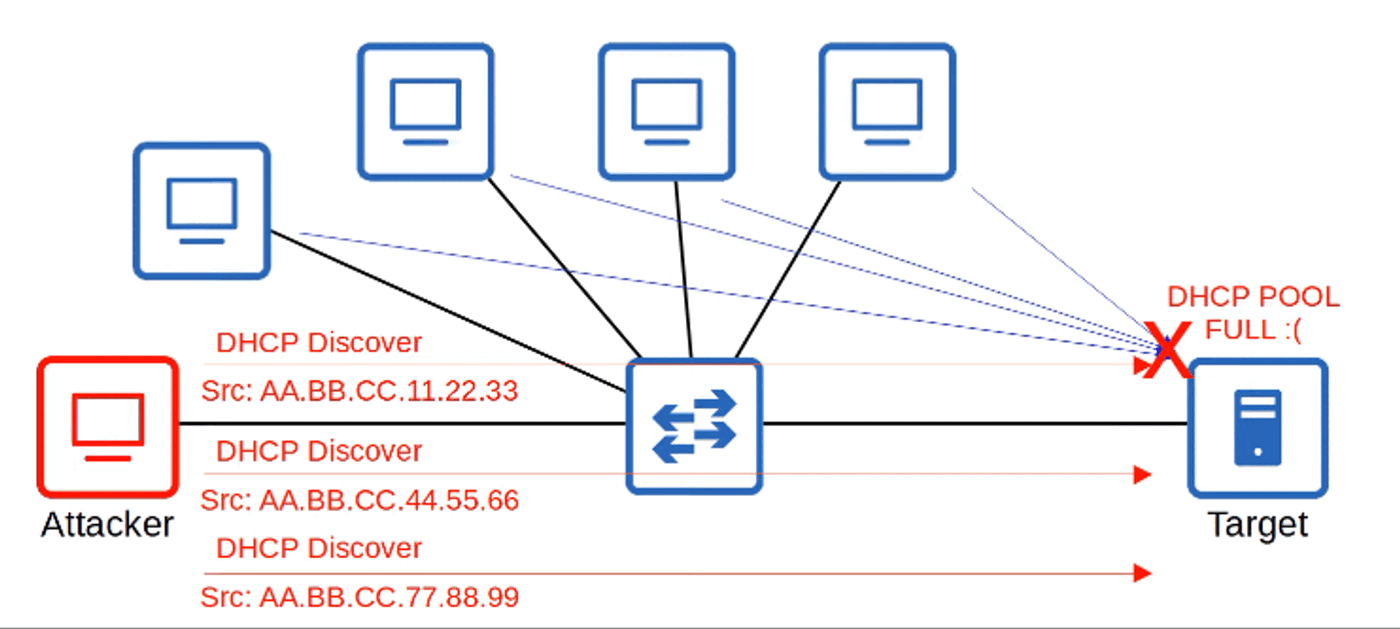
\includegraphics[keepaspectratio,alt={image}]{images/49-security-fundamentals/img-003.png}}
\end{figure}

\section{Reflection / Amplification
Attacks}\label{reflection-amplification-attacks}

\begin{itemize}
\item
  In a REFLECTION attack, the ATTACKER sends traffic to a
  \emph{reflector}, and spoofs the SOURCE of the PACKET using the
  TARGET'S IP ADDRESS
\item
  The \emph{reflector} (ie: a DNS Server) sends the reply to the
  TARGET'S IP ADDRESS
\item
  If the amount of traffic sent to the TARGET is large enough, this can
  result in a Denial-of-Service
\item
  A REFLECTION attack becomes an AMPLIFICATION attack when the amount of
  traffic sent by the ATTACKER is small but it triggers a LARGE amount
  of traffic to be sent from the \emph{reflector} to the TARGET
\end{itemize}

\begin{figure}
\centering
\pandocbounded{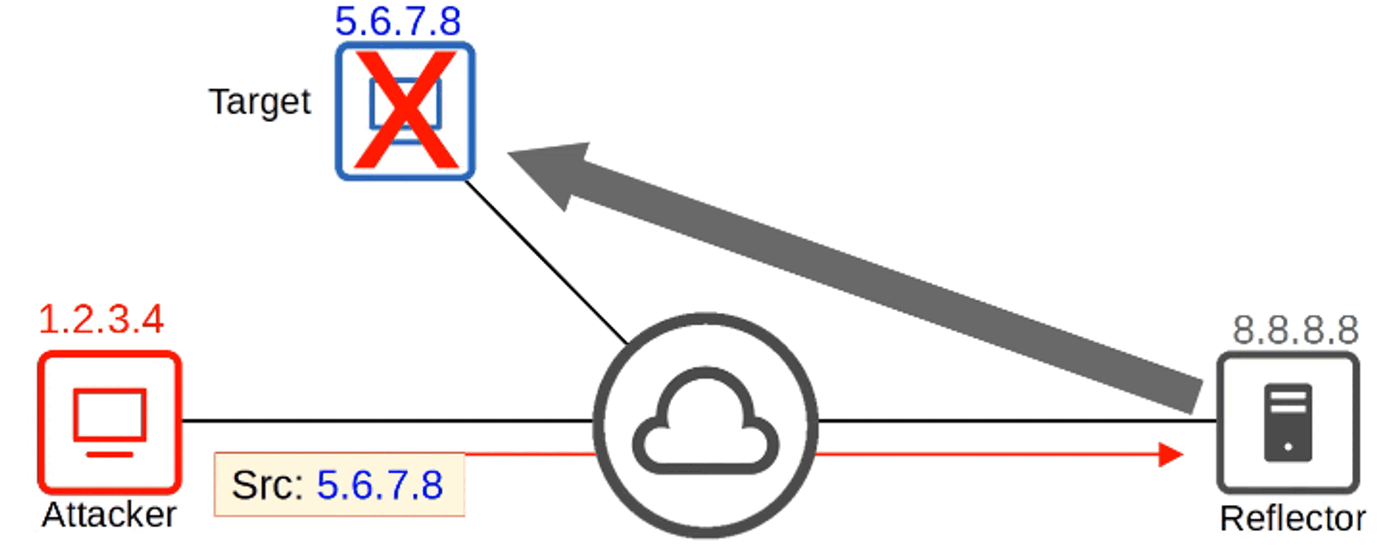
\includegraphics[keepaspectratio,alt={image}]{images/49-security-fundamentals/img-004.png}}
\end{figure}

\section{Man-in-the-Middle Attacks}\label{man-in-the-middle-attacks}

\begin{itemize}
\tightlist
\item
  In a MAN-IN-THE-MIDDLE attack, the ATTACKER places himself between the
  SOURCE and DESTINATION to eavesdrop on communications, or to modify
  traffic before it reaches the DESTINATION
\item
  A common example is ARP SPOOFING, also known as ARP POISONING
\item
  A HOST sends an ARP REQUEST, asking for the MAC ADDRESS of another
  DEVICE
\item
  The TARGET of the request sends an ARP REPLY, informing the requester
  of it's MAC ADDRESS
\item
  The ATTACKER waits and sends another ARP REPLY after it's legitimate
  replier
\end{itemize}

\begin{figure}
\centering
\pandocbounded{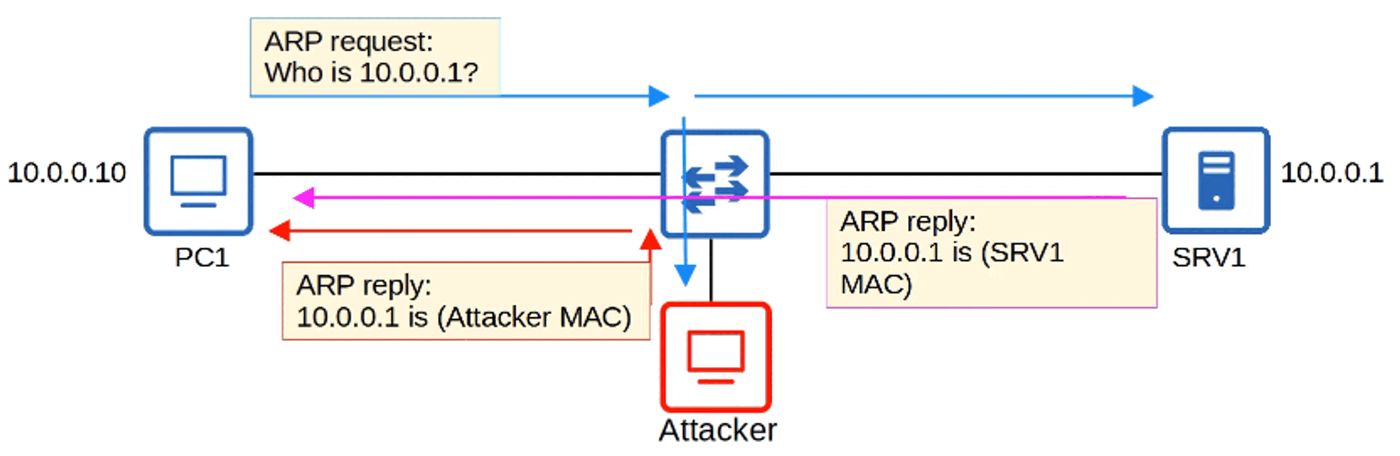
\includegraphics[keepaspectratio,alt={image}]{images/49-security-fundamentals/img-005.png}}
\end{figure}

\begin{itemize}
\tightlist
\item
  In PC1's ARP table, the entry for 10.0.0.1 will have the ATTACKER'S
  MAC ADDRESS
\item
  When PC1 tries to send traffic to SRV1, it will be forwarded to the
  ATTACKER instead
\item
  The ATTACKER can inspect the messages, and then forward them on to
  SRV1
\item
  The ATTACKER can also modify the messages before forwarding them to
  SRV1
\item
  This compromises the CONFIDENTIALITY and INTEGRITY of communication
  between PC1 and SRV1
\end{itemize}

\begin{figure}
\centering
\pandocbounded{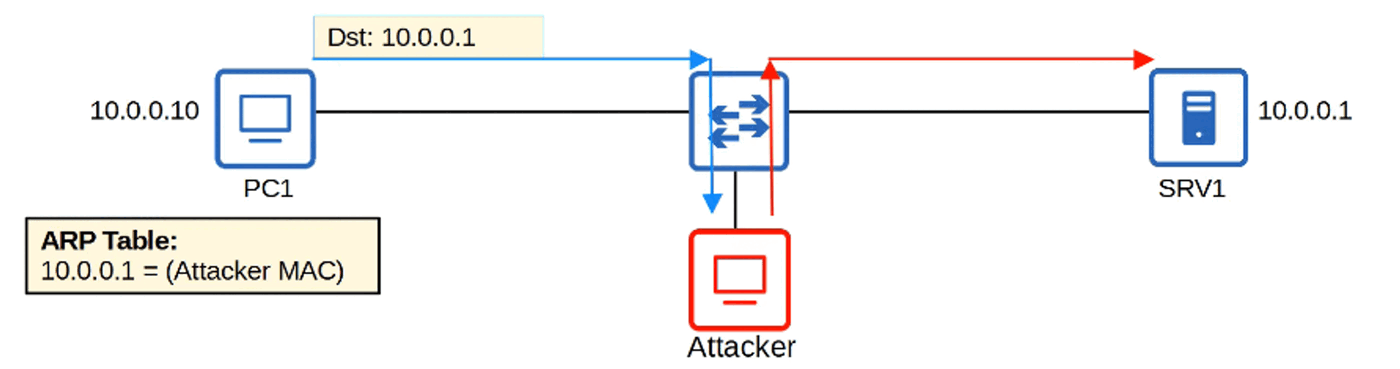
\includegraphics[keepaspectratio,alt={image}]{images/49-security-fundamentals/img-006.png}}
\end{figure}

\section{Reconnaissance Attacks}\label{reconnaissance-attacks}

\begin{itemize}
\tightlist
\item
  RECONNAISSANCE ATTACKS are not attacks themselves but they are used to
  gather information about a TARGET which can be used for a future
  attack
\item
  This is often publicly available information
\item
  IE: nslookup to learn the IP ADDRESS of a site
\end{itemize}

\begin{figure}
\centering
\pandocbounded{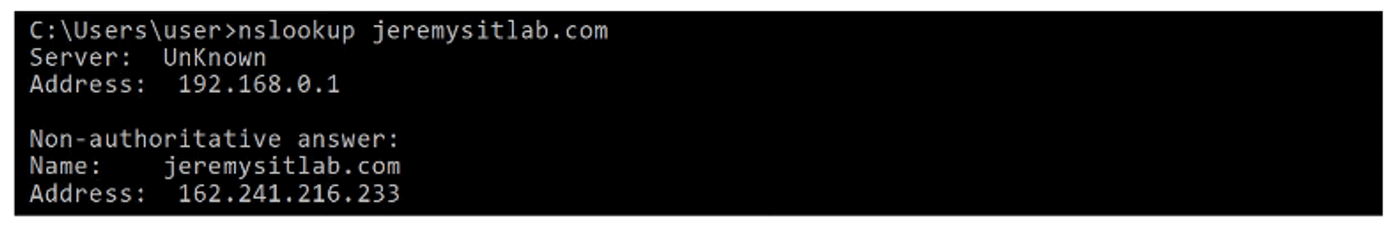
\includegraphics[keepaspectratio,alt={image}]{images/49-security-fundamentals/img-007.png}}
\end{figure}

\begin{itemize}
\tightlist
\item
  Or a WHOIS query to learn email addresses, phone numbers, physical
  addresses, etc.
\end{itemize}

\url{https://lookup.icann.org/lookup}

\section{Malware}\label{malware}

\begin{itemize}
\item
  MALWARE (MALICIOUS SOFTWARE) refers to a variety of harmful programs
  that can infect a computer
\item
  VIRUSES infect other software (a `host program')

  \begin{itemize}
  \tightlist
  \item
    The VIRUS spreads as the software is shared by USERS. Typically,
    they CORRUPT or MODIFY files on the TARGET computer
  \end{itemize}
\item
  WORMS do not require a host program. They are standalone malware and
  they are able to spread on their own, without user interaction. They
  spread of WORMS can congest the NETWORK but the `payload' of a WORM
  can cause additional harm to TARGET DEVICES
\item
  TROJAN HORSES are harmful software that is disguised as LEGITIMATE
  software. They are spread through user interaction such as opening
  email attachments, downloading a file from the Internet.
\end{itemize}

The above MALWARE types can exploit various VULNERABILITIES to threaten
any of the CIA of a TARGET DEVICE

** There are MANY types of MALWARE

\section{Social Engineering Attacks}\label{social-engineering-attacks}

\begin{itemize}
\item
  SOCIAL ENGINEERING ATTACKS target the most vulnerable part of ANY
  system - PEOPLE!
\item
  They involve psychological manipulation to make the TARGET reveal
  confidential information or perform some action
\item
  PHISHING typically involves fraudulent emails that appear to come from
  a legitimate business (Amazon, bank, credit card company, etc) and
  contain links to a fraudulent website that seems legitimate. Users are
  told to login to the fraudulent website, providing their login
  credentials to the attacker.

  \begin{itemize}
  \tightlist
  \item
    SPEAR PHISHING is a more targeted form of phishing, ie: aimed at
    employees of a certain company
  \item
    WHALING is a phishing targeted at high-profile individuals, ie: a
    company president
  \end{itemize}
\item
  VISHING (Voice Phishing) is phishing performed over a phone
\item
  SMISHING (SMS Phishing) is phishing using SMS text messages
\item
  WATERING HOLE attacks compromise sites that the TARGET victim
  frequently visits. If a malicious link is placed on a website the
  TARGET trusts, they might not hesitate to click it
\item
  TAILGATING attack involves entering restricted, secured areas by
  simply walking in behind an authorized person as they enter. Often the
  TARGET will hold the door open for the ATTACKER to be polite, assuming
  the ATTACKER is also authorized to enter.
\end{itemize}

\section{Password-Related Attacks}\label{password-related-attacks}

\begin{itemize}
\tightlist
\item
  Most systems use a USERNAME / PASSWORD combination to AUTHENTICATE
  users
\item
  The USERNAME is often simple / easy to guess (for example the user's
  email address) and the strength and secrecy of the password is relied
  on to provide the necessary security
\item
  ATTACKERS can learn a user's passwords via multiple methods:

  \begin{itemize}
  \tightlist
  \item
    Guessing
  \item
    DICTIONARY ATTACK :

    \begin{itemize}
    \tightlist
    \item
      A program runs through a `dictionary' or list of common words /
      passwords to find the TARGET'S password
    \end{itemize}
  \item
    BRUTE FORCE ATTACK :

    \begin{itemize}
    \tightlist
    \item
      A program tries every possible combination of letters, numbers,
      and special characters to find the TARGET'S password
    \end{itemize}
  \end{itemize}
\item
  STRONG PASSWORDS should contain:

  \begin{itemize}
  \tightlist
  \item
    At LEAST 8 characters (preferably more)
  \item
    A mixture of UPPERCASE and LOWERCASE letters
  \item
    A mixture of LETTERS and NUMBERS
  \item
    One of more SPECIAL CHARACTERS (\# @ ! ? etc.)
  \item
    Should be CHANGED REGULARLY
  \end{itemize}
\end{itemize}

\section{Passwords / Multi-Factor Authentication
(MFA)}\label{passwords-multi-factor-authentication-mfa}

\begin{itemize}
\tightlist
\item
  MULTI-FACTOR AUTHENTICATION involves providing more than just a
  USERNAME / PASSWORD to prove your identity
\item
  It usually involves providing TWO of the following ( = Two-Factor
  Authentication) :

  \begin{itemize}
  \tightlist
  \item
    SOMETHING YOU KNOW

    \begin{itemize}
    \tightlist
    \item
      A USERNAME / PASSWORD combination, a PIN, etc.
    \end{itemize}
  \item
    SOMETHING YOU HAVE

    \begin{itemize}
    \tightlist
    \item
      Pressing a notification that appears on your phone, a badge that
      is scanned, etc.
    \end{itemize}
  \item
    SOMETHING YOU ARE

    \begin{itemize}
    \tightlist
    \item
      Biometrics such as a face scan, palm scan, fingerprint scan,
      retina scan, etc.
    \end{itemize}
  \end{itemize}
\item
  Requiring multiple factors of AUTHENTICATION greatly increases the
  security. Even if the ATTACKER learns the TARGET'S PASSWORD (SOMETHING
  YOU KNOW), they won't be able to login to the TARGET'S account
\end{itemize}

\section{Digital Certificates}\label{digital-certificates}

\begin{itemize}
\tightlist
\item
  DIGITAL CERTIFICATES are another form of AUTHENTICATION used to prove
  the identity of the holder of the certificate
\item
  They are used for websites to verify that the website being accessed
  is legitimate
\item
  Entities that want a certificate to prove their identity send a CSR
  (CERTIFICATE SIGNING REQUEST) to a CA (CERTIFICATE AUTHORITY) which
  will generate and sign the certificate
\end{itemize}

\section{Controlling and Monitoring Users with
AAA}\label{controlling-and-monitoring-users-with-aaa}

\begin{itemize}
\item
  AAA (Triple-A) stands for AUTHENTICATION, AUTHORIZATION, and
  ACCOUNTING
\item
  It is a framework for controlling and monitor users of a computer
  system (ie: a network)
\item
  AUTHENTICATION

  \begin{itemize}
  \tightlist
  \item
    Process of verifying a user's identity
  \item
    Logging in = AUTHENTICATION
  \end{itemize}
\item
  AUTHORIZATION

  \begin{itemize}
  \tightlist
  \item
    Process of granting the user the appropriate access and permissions
  \item
    Granting the user access to some files / services, restricting
    access to other files / services = AUTHORIZATION
  \end{itemize}
\item
  ACCOUNTING

  \begin{itemize}
  \tightlist
  \item
    Process of recording the user's activities on the system
  \item
    Logging when a user makes a change to a file = ACCOUNTING
  \end{itemize}
\item
  Enterprises typically use a AAA server to provide AAA services

  \begin{itemize}
  \tightlist
  \item
    ISE (Identity Services Engine) is Cisco's AAA server
  \end{itemize}
\item
  AAA Servers usually support the following TWO AAA Protocols:

  \begin{itemize}
  \tightlist
  \item
    RADIUS : Open Standard Protocol

    \begin{itemize}
    \tightlist
    \item
      Uses UDP PORTS 1812 and 1813
    \end{itemize}
  \item
    TACACS+ : Cisco Proprietary Protocol

    \begin{itemize}
    \tightlist
    \item
      Uses TCP PORT 49
    \end{itemize}
  \end{itemize}
\end{itemize}

\begin{tipbox}

FOR THE CCNA, KNOW THE DIFFERENCES BETWEEN AUTHENTICATION,
AUTHORIZATION, and ACCOUNTING

\end{tipbox}

\section{Security Program Elements}\label{security-program-elements}

\begin{itemize}
\tightlist
\item
  USER AWARENESS PROGRAMS are designed to make employees aware of
  potential security threats and risks
\item
  USER TRAINING PROGRAMS are formal than USER AWARENESS PROGRAMS
\item
  PHYSICAL ACCESS CONTROL protect equipment and data from potential
  attackers by only allowing authorized users into the protected areas
  such as NETWORK CLOSETS or DATA CENTER FLOORS
\end{itemize}
